\documentclass[ASNA,twocolumn]{USG}
\usepackage{anyfontsize}
\usepackage{amsmath,amssymb,bm,mathtools}
\usepackage{graphicx}
\usepackage{booktabs}
\usepackage{microtype}
\usepackage{siunitx}
\usepackage{xcolor}
\usepackage{url}
\graphicspath{{../manuscript/figures/}}
\newcommand{\Tr}{\operatorname{Tr}}
\newcommand{\deff}{d_{\mathrm{eff}}}

\articletype{RESEARCH ARTICLE}
\journal{Advanced Quantum Technologies}
\volume{0}
\copyyear{2026}
\startpage{1}
\articledoi{}

\begin{document}

\title{Spectral Orientation of Measurement-Accessible Quantum Tangent Geometry in Variational Quantum Circuits}
\author[1]{Marwan Ait Haddou}[https://orcid.org/0009-0008-1734-1721]
\authormark{AIT HADDOU}
\titlemark{SPECTRAL ORIENTATION OF MEASUREMENT-ACCESSIBLE QUANTUM TANGENT GEOMETRY}
\address[1]{Independent Researcher}
\corres{Marwan Ait Haddou (\email{aithaddou.marwan@outlook.com})}
\keywords{variational quantum circuits | quantum information geometry | quantum measurements | readout design | Fisher information | quantum machine learning}

\abstract[ABSTRACT]{After a fixed measurement of a trainable variational quantum circuit, readout subspaces of the same dimension can retain different amounts of parameter-tangent information. This dependence is resolved by the covariance spectrum of Fisher-normalized measurement scores and by the orientation of the retained readout subspace within that score space. Random rank-matched subspaces provide a rank-only reference. Across five generic circuit families, one- and two-body diagonal readouts remain near this reference through 16 qubits although the tangent covariance becomes strongly anisotropic. For Haar-$U(4)$ circuits at 12 qubits, a cross-fitted aligned readout of the same rank as the physical one-body readout increases the mean directional gradient-energy proxy by a factor of 9.584 and the finite-shot signal-to-noise ratio by a factor of 3.111. A random rank-matched subspace remains near the reference. A half-filled $U(1)$-conserving family shows a different regime in which low-weight $Z$ readouts are already aligned with leading tangent directions. Spectral orientation therefore determines how much measured parameter-tangent information remains accessible after readout restriction and can alter finite-shot directional signal without changing the quantum measurement or readout rank.}

\maketitle

\section{Introduction}

Variational quantum circuits interact with classical learning and control loops through measured data. Quantum Fisher information (QFI) and related state-space metrics characterize local changes of a parameterized quantum state before a measurement is specified \cite{BraunsteinCaves1994,Stokes2020,Haug2021}. A fixed measurement restricts this geometry to the information carried by its outcome distribution. Retaining only selected observables or classical features imposes a second restriction on the same measurement record \cite{BraunsteinCaves1994,HottaOzawa2004,LuLuoOh2012}. The present work studies this readout stage while keeping the quantum measurement fixed.

Measurement-limited visibility also appears in other quantum-learning settings. Gross and Rieser formulate quantum extreme learning machines through Pauli-transfer matrices and characterize which encoded Pauli features can be reconstructed from the row space exposed by reservoir dynamics and measured observables \cite{GrossRieser2026}. Their local-injectivity condition asks whether the effective readout map remains injective on the tangent space of the classical input feature map. The object considered here is different. The circuit parameters themselves are varied, the resulting probability derivatives are represented as Fisher-normalized scores after a fixed measurement, and the readout is evaluated by how much of the covariance of these parameter tangents it retains. The resulting question is therefore differential and parameter-geometric rather than a Pauli-feature decoding problem.

Let $u_v$ denote a normalized measurement-score vector for a parameter-space direction $v$, and let
\begin{equation}
C=\mathbb{E}_v[u_vu_v^{\mathsf T}],
\qquad C\succeq0,
\qquad \operatorname{Tr}C=1,
\end{equation}
be the covariance of these tangent directions in an $N$-dimensional centered score space. A retained readout span is represented by an orthogonal projector $P$ of rank $r$. Its mean retained tangent mass is
\begin{equation}
R(P,C)=\operatorname{Tr}(PC),
\qquad
\rho(P,C)=\frac{\operatorname{Tr}(PC)}{r/N}.
\label{eq:aqt-intro-rho}
\end{equation}
Here $r/N$ is the mean overlap for a rank-$r$ subspace under random relative orientation. It serves as a rank-only reference; it is not an assumption that a physical circuit or readout is Haar-oriented.

The isotropic limit supplies a useful boundary case. A companion analysis derives exact finite-size readout-rank laws when the joint state--tangent frame is isotropic \cite{AitHaddou2026IsotropicRankLaws}. The present paper addresses the regime in which that assumption is absent. For an arbitrary trace-one covariance, the rank fixes the random-orientation mean, the eigenvalue spectrum determines the width of the random-orientation distribution, and the orientation of the physical readout relative to the covariance eigenspaces determines the observed retention. The effective spectral dimension
\begin{equation}
 d_{\mathrm{eff}}(C)=\frac{1}{\operatorname{Tr}(C^2)}
\end{equation}
quantifies spectral concentration. Standard Grassmann projector moments \cite{CollinsMatsumoto2017,Bendokat2024} give a null variance bounded by $2/(r d_{\mathrm{eff}})$. A readout can therefore lie near its rank reference even when $d_{\mathrm{eff}}/N$ is small. Near-rank retention is not evidence of isotropic tangent geometry.

The numerical study tests this distinction with computational-basis measurement and low-weight diagonal $Z$ readouts across several variational circuit families. Family-balanced generic circuits remain close to the rank reference for one- and two-body readouts over the tested sizes while their tangent covariance becomes strongly anisotropic. Architecture-resolved deviations show that this aggregate behavior is not literal Haar orientation. The decisive control keeps the circuit, measurement record, readout rank, and evaluation resources fixed while changing only the retained score subspace. In Haar-$U(4)$ circuits, a cross-fitted leading tangent subspace retains substantially more tangent mass than the physical one-body span at the same rank. The difference persists in finite-shot directional-signal diagnostics, whereas an independent random rank-matched subspace remains close to the rank baseline.

A half-filled $U(1)$-conserving RZ--XY family provides a structured contrast. Its low-weight diagonal readout is already strongly aligned with leading tangent directions, including after the random-orientation reference is corrected to the fixed-charge score sector. A symmetry-breaking pilot suppresses this alignment, but the data do not identify a unique microscopic mechanism. Readout--charge compatibility, fixed-charge harmonic geometry, restricted controllability, and slow modes under conservation remain distinct possible contributions. The reported finite-size fits are used only to describe the tested range and are not interpreted as asymptotic or hydrodynamic exponents.

The contribution is a rank-controlled spectral description of measurement-accessible parameter tangents in trainable variational circuits. Standard random-subspace identities and the Ky Fan variational principle are used as reference tools rather than novelty claims. The new evidence is the combination of covariance-resolved orientation diagnostics, physical/random/cross-fitted readouts at equal rank, a sector-corrected structured case study, and a finite-shot operational comparison. These results identify readout orientation as a design variable at the quantum-measurement/classical-processing interface. They do not by themselves establish supervised-loss trainability or a barren-plateau theorem; those questions additionally depend on the task gradient, classical postprocessing, and optimization dynamics.

\section{Measurement-Accessible Parameter-Tangent Geometry}

\subsection{Normalized tangent scores}

Let $p_\theta(x)$ denote the outcome distribution of a fixed quantum measurement applied to a parameterized state $\rho_\theta$. For a parameter-space direction $v$, the derivative $\partial_v p_\theta(x)$ defines a tangent to the classical probability simplex. On the regular support, the Fisher-weighted tangent is
\begin{equation}
 s_v(x)=\frac{\partial_v p_\theta(x)}{\sqrt{p_\theta(x)}}.
\label{eq:aqt-score}
\end{equation}
Probability normalization removes the constant mode. After normalizing each nonzero tangent,
\begin{equation}
 u_v=\frac{s_v}{\|s_v\|_2},
\qquad \|u_v\|_2=1,
\end{equation}
the ensemble of parameter directions defines the trace-one covariance
\begin{equation}
 C=\mathbb E_v[u_vu_v^{\mathsf T}],
\qquad C\succeq0,
\qquad \operatorname{Tr}C=1.
\label{eq:aqt-C}
\end{equation}
Before this unit normalization, $\|s_v\|_2^2$ is the classical Fisher information carried by the fixed measurement along $v$ \cite{BraunsteinCaves1994,LuLuoOh2012}. The covariance $C$ therefore describes the distribution of measurement-visible tangent \emph{directions} after their overall Fisher scale has been factored out.

The eigenvectors of $C$ identify score-space directions that repeatedly carry parameter-tangent variation. Spectral concentration is summarized by
\begin{equation}
 d_{\mathrm{eff}}(C)=\frac{1}{\operatorname{Tr}(C^2)}.
\label{eq:aqt-deff}
\end{equation}
The isotropic covariance $I/N$ has $d_{\mathrm{eff}}=N$; smaller values indicate concentration into fewer score directions.

\subsection{Readout restriction as a projector}

A retained family of linear observables or score features spans a subspace of the centered score space. Let $P=P^{\mathsf T}=P^2$ project onto this span and let $r=\operatorname{Tr}P$. For a normalized tangent $u_v$, the fraction retained by the readout is $\|Pu_v\|_2^2$. Averaging over the tangent ensemble gives
\begin{equation}
 R(P,C)=\mathbb E_v\|Pu_v\|_2^2
       =\operatorname{Tr}(PC).
\label{eq:aqt-retention}
\end{equation}
The quantity $R$ is therefore the mean normalized tangent mass visible to the retained readout. The quantum state family and measurement are unchanged when $P$ is changed; only the classical subspace retained from the same measurement record is modified.

This parameter-tangent formulation differs from feature-decoding analyses of fixed quantum reservoirs. In the Pauli-transfer description of quantum extreme learning machines, the relevant projector acts on encoded Pauli-feature directions exposed by reservoir dynamics and the measured observables \cite{GrossRieser2026}. Here the projected vectors are Fisher-normalized derivatives with respect to trainable circuit parameters after a fixed measurement. The object of interest is their covariance $C$ and its orientation relative to the readout span.

\begin{figure*}[t]
\centering
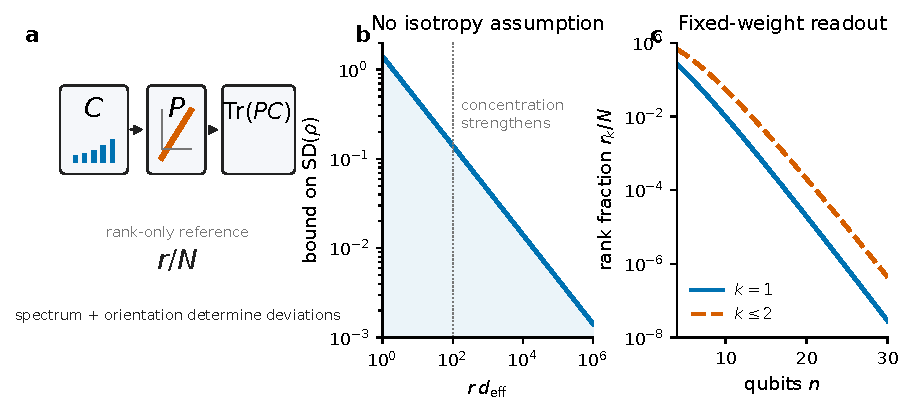
\includegraphics[width=.96\textwidth]{fig1_framework_theory.pdf}
\caption{Measurement-accessible parameter-tangent geometry. A fixed quantum measurement defines a centered score space. The tangent-score covariance $C$ distributes normalized parameter-tangent mass within that space, while a rank-$r$ readout projector $P$ selects the retained directions. The mean retained mass is $R=\operatorname{Tr}(PC)$. Random relative orientation supplies the rank-only reference $r/N$; the covariance spectrum sets the corresponding null width, and the physical orientation of $P$ determines the observed deviation.}
\label{fig:framework-aqt}
\end{figure*}

\section{Rank Reference and Spectral Orientation}

\subsection{Random relative orientation}

To separate readout dimension from orientation, $C$ is held fixed while a rank-$r$ projector is drawn uniformly from the real Grassmann manifold $\mathrm{Gr}(r,N)$. Rotational invariance gives
\begin{equation}
 \mathbb E_P P=\frac{r}{N}I,
 \qquad
 \mathbb E_P R(P,C)=\frac{r}{N}.
\end{equation}
The rank-normalized retention is
\begin{equation}
 \rho(P,C)=\frac{\operatorname{Tr}(PC)}{r/N},
\label{eq:aqt-rho}
\end{equation}
so that $\mathbb E_P\rho=1$. This is a random-orientation reference, not a physical model of the circuits studied below. The same mean appears in the exact isotropic readout-rank law derived in the companion isotropic analysis \cite{AitHaddou2026IsotropicRankLaws}.

Standard Grassmann projector moments give
\begin{equation}
\operatorname{Var}_P(\rho\mid C)=
\frac{2(N-r)\left[N\operatorname{Tr}(C^2)-1\right]}
{r(N-1)(N+2)}
\le \frac{2}{r d_{\mathrm{eff}}(C)}.
\label{eq:aqt-var}
\end{equation}
The derivation is given in the Supporting Information. Equation~\eqref{eq:aqt-var} is used only as a null-width calculation. It shows that retention can concentrate near the rank reference whenever $r d_{\mathrm{eff}}$ is large, even when $d_{\mathrm{eff}}/N$ is small. A value $\rho\approx1$ therefore does not imply an isotropic tangent covariance.

For computational-basis measurement with full support, the centered score dimension is $N=2^n-1$. A cumulative diagonal Pauli-$Z$ readout through fixed weight $k$ has rank $r_{\le k}=\sum_{j=1}^k\binom nj$. The resulting ratio $r_{\le k}/N$ is used only to set the rank scale. The exact isotropic law and its finite-size distributions belong to the companion rank-law analysis \cite{AitHaddou2026IsotropicRankLaws}; the present work tests what determines retention when the tangent covariance is not isotropic.

\subsection{Same-rank spectral controls}

For a fixed covariance with eigenvalues $\lambda_1\ge\cdots\ge\lambda_N$, the Ky Fan principle gives the maximal rank-$r$ retention
\begin{equation}
 \max_{\operatorname{rank}(P)=r}\operatorname{Tr}(PC)
 =\sum_{j=1}^{r}\lambda_j.
\label{eq:aqt-kyfan}
\end{equation}
This standard result \cite{KyFan1949} provides an optimistic spectral benchmark. The operational aligned readout is instead cross-fitted: its leading rank-$r$ score subspace is estimated from an independent calibration ensemble and evaluated on held-out tangents. This prevents the same tangent samples from both selecting and evaluating the subspace.

Three readouts are compared at identical rank: the physical low-weight span, an independent random rank-matched subspace, and the cross-fitted aligned subspace. Differences among these controls isolate orientation at fixed dimension.

\section{Numerical Protocol}

The numerical campaign uses computational-basis measurement and diagonal $Z$ readouts. Five nonconserving circuit families form the generic ensemble: RY--RZ--CZ, SU2--CNOT, SU2--CZ ring, random-matching SU2--CZ, and Haar-$U(4)$ brickwork. A half-filled number-conserving RZ--XY family supplies the structured $U(1)$ case study. Exact circuit definitions, depths, system sizes, frozen seeds, and generated circuit diagrams are provided in the Supporting Information and reproducibility repository \cite{Bergholm2018,AitHaddou2026MeasurementAccessible}.

A circuit instance is the independent statistical unit. Tangent directions generated within one circuit are used to estimate its score covariance and readout statistics but are not treated as independent bootstrap replicates. Confidence intervals are obtained by nonparametric bootstrap over circuit instances \cite{Efron1979}. Generic aggregates are family-balanced so that no architecture is weighted by its number of available samples.

The cross-fitted operational profile uses 128 calibration tangents and 128 independent evaluation tangents per circuit. Generic Haar-$U(4)$ cells use 16 circuit instances per size and the $U(1)$ cells use 20. Finite-shot evaluation uses a multinomial measurement model with $10^4$ shots and eight held-out finite-difference directions. The calibration ensemble is a separate resource. It is not counted as free measurement cost in the fixed-evaluation-budget comparison, and a hardware implementation would need to account for its shot or derivative-query cost separately.

\section{Rank-Typical Retention Can Coexist with Strong Anisotropy}

For the family-balanced generic ensemble, physical one- and two-body readouts remain close to the rank reference through $n=16$. A targeted Haar-$U(4)$ stress test at $n=18$ gives
\begin{equation}
 \rho_1=0.929\;[0.910,0.950],
 \qquad
 \rho_2=0.958\;[0.952,0.966].
\label{eq:aqt-n18-rho}
\end{equation}
The $n=18$ point is a single-architecture stress test rather than the family-balanced estimator used at smaller sizes \cite{AitHaddou2026MeasurementAccessible}.

The covariance is nevertheless far from isotropic. The normalized purity $N\operatorname{Tr}(C^2)$ rises from approximately $1.35$ at $n=6$ to $6.17$ at $n=12$, $17.52$ at $n=14$, and $49.84$ at $n=16$. Correspondingly, $d_{\mathrm{eff}}/N$ falls from $0.746$ at $n=6$ to $0.1767$ at $n=12$ and $0.0233$ at $n=16$. The Haar-$U(4)$ stress point at $n=18$ has normalized purity about $146.8$ and $d_{\mathrm{eff}}/N\approx0.00683$ \cite{AitHaddou2026MeasurementAccessible}. Near-rank retention therefore persists while tangent mass becomes concentrated into a small spectral fraction of the score space.

Architecture-resolved data show that this agreement is not literal random orientation. The RY--RZ--CZ family develops a one-body deficit, with mean $\rho_1\simeq0.874$ at $n=14$ and $0.877$ at $n=16$. Its full computational-basis Fisher fraction remains of order one, so the deficit occurs at the readout projection rather than through disappearance of the measured tangent signal. No microscopic gate-level mechanism is assigned to this architecture-specific deviation.

\begin{figure*}[t]
\centering
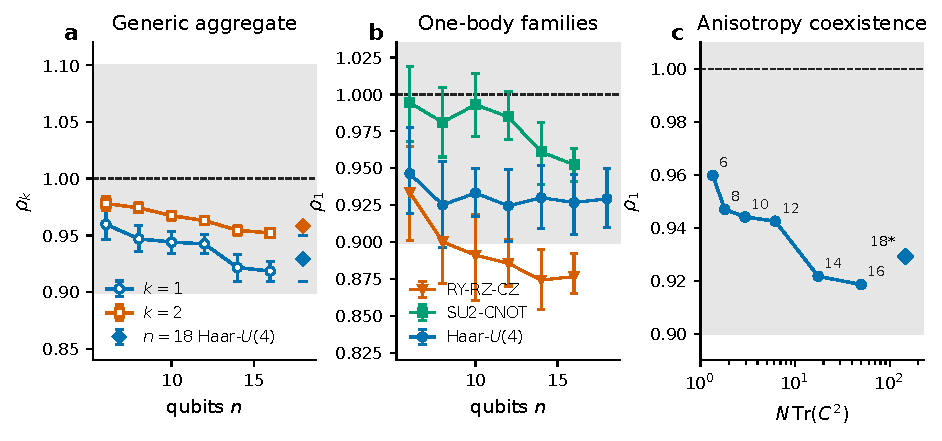
\includegraphics[width=.96\textwidth]{fig2_rank_architecture_anisotropy.pdf}
\caption{Rank-normalized retention and covariance anisotropy. Family-balanced generic low-weight readouts remain close to the random-orientation rank reference over the tested sizes while the normalized purity $N\operatorname{Tr}(C^2)$ grows and $d_{\mathrm{eff}}/N$ decreases. Architecture-resolved deviations show that near-rank aggregate retention is not evidence of isotropic or Haar-oriented tangent geometry.}
\label{fig:rank-aqt}
\end{figure*}

\section{Equal Rank Does Not Imply Equal Accessibility}

The direct test of orientation compares subspaces with identical rank. For Haar-$U(4)$ circuits at $n=12$, the physical one-body readout retains
\begin{equation}
 R_{\mathrm{phys}}=2.71\times10^{-3},
\end{equation}
whereas the cross-fitted aligned subspace retains
\begin{equation}
 R_{\mathrm{xfit}}=3.06\times10^{-2}.
\end{equation}
The same-sample Ky Fan benchmark is $9.15\times10^{-2}$ \cite{AitHaddou2026MeasurementAccessible}. Thus the low retention of the physical readout is not imposed by its rank; substantially more tangent mass is available within another subspace of the same dimension.

The half-filled $U(1)$ circuit occupies a different spectral regime. At $n=12$, the physical one-body readout retains $0.292$, the cross-fitted aligned subspace $0.375$, and the Ky Fan benchmark $0.444$. The physical readout is not optimal, but it is already close to the leading tangent directions compared with the generic Haar-$U(4)$ case.

The physical, random rank-matched, cross-fitted aligned, and Ky Fan comparisons should be interpreted differently. The physical readout represents the experimentally chosen low-weight feature span. The random control sets an orientation null. Cross-fitting estimates a realizable aligned subspace without evaluating on its calibration tangents. The Ky Fan value is an upper benchmark and is not an operational estimator.

\begin{figure*}[t]
\centering
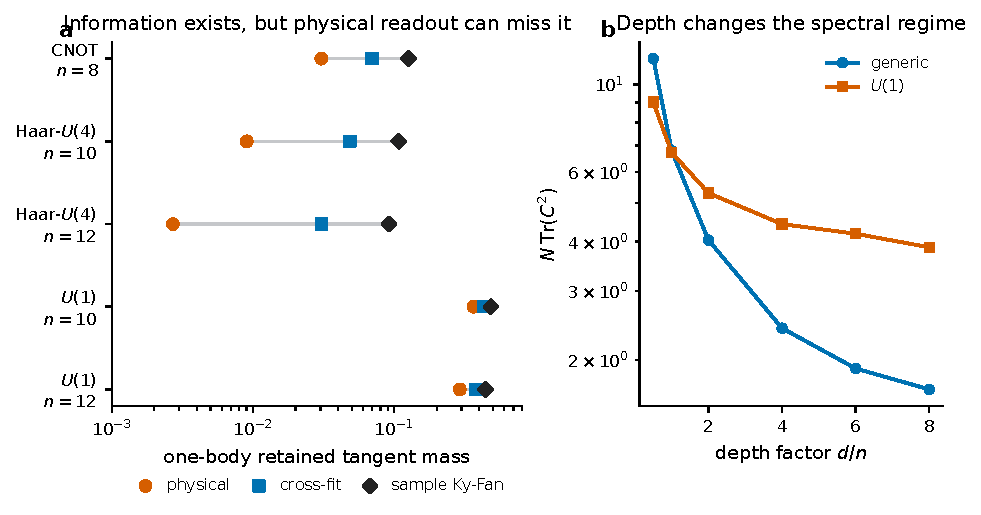
\includegraphics[width=.96\textwidth]{fig4_spectral_mechanism_depth.pdf}
\caption{Equal-rank spectral comparison. Physical low-weight, cross-fitted aligned, and same-sample Ky Fan subspaces have the same retained dimension but can capture different amounts of tangent mass. The orientation gap is large in generic Haar-$U(4)$ circuits and smaller in the half-filled $U(1)$ family, where the physical low-weight readout is already closer to the leading tangent subspace.}
\label{fig:spectrum-aqt}
\end{figure*}

\section{Finite-Shot Consequence of Readout Orientation}

The same-rank comparison is repeated with directional signal and finite-shot noise while holding the circuit, computational-basis measurement record, readout rank, evaluation tangents, and evaluation shot budget fixed. For a direction $v$, the raw retained Fisher energy is proportional to $F_{\mathrm{full}}(v)\|Pu_v\|_2^2$. Combining this quantity with the multinomial covariance of the measurement record yields the finite-shot signal-to-noise ratio used below. Full definitions are given in the Supporting Information.

For Haar-$U(4)$ circuits, replacing the physical one-body span with the cross-fitted aligned subspace increases the mean directional gradient-energy proxy by factors
\begin{equation}
 2.963,\quad 4.639,\quad 9.584
\end{equation}
for $n=8,10,12$. The corresponding finite-shot signal-to-noise gains are
\begin{equation}
 1.734,\quad 2.125,\quad 3.111.
\end{equation}
An independent random rank-matched subspace remains near the physical generic baseline \cite{AitHaddou2026MeasurementAccessible}. The improvement therefore follows from orientation within the same measurement-induced score space rather than from additional observables or a larger evaluation shot budget.

The $U(1)$ family leaves less room for improvement because its physical readout is already aligned. At $n=8,10,12$, the aligned-to-physical gradient-energy ratios are approximately $1.148$, $1.189$, and $1.210$, with signal-to-noise gains $1.068$, $1.097$, and $1.112$. These quantities are directional diagnostics, not supervised-loss gradient variances. No labels, classical prediction head, or optimization trajectory enter this comparison.

\begin{figure*}[t]
\centering
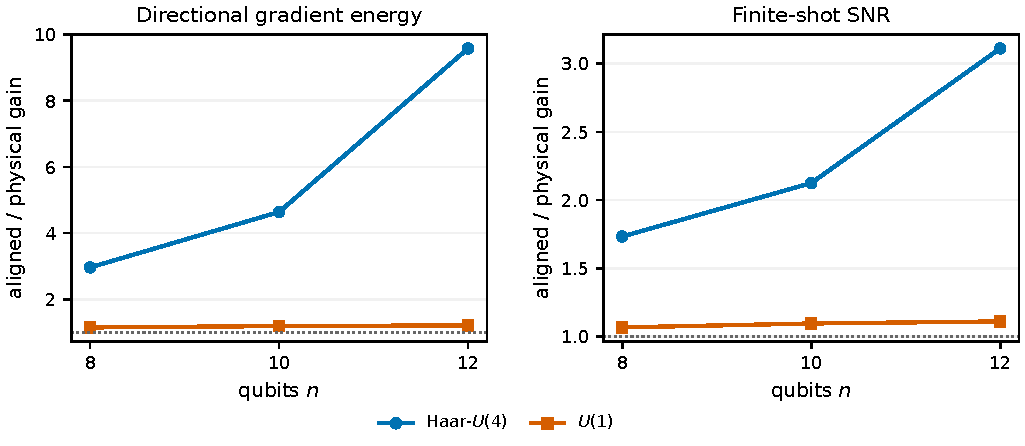
\includegraphics[width=.94\textwidth]{appendix_operational_gains.pdf}
\caption{Finite-shot consequence of equal-rank readout orientation. The panels compare the physical and cross-fitted aligned readouts at fixed circuit, computational-basis measurement, readout rank, evaluation directions, and shot budget. Generic Haar-$U(4)$ circuits show increasing directional gradient-energy and signal-to-noise gains with system size, whereas the structured $U(1)$ readout leaves less room for orientation improvement.}
\label{fig:operational-aqt}
\end{figure*}

\section{Structured Low-Weight Alignment in a Half-Filled $U(1)$ Circuit}

The half-filled RZ--XY circuit retains much more low-weight tangent mass than the full-space rank scale would suggest. At $n=18$, the one-body retention is approximately $0.215$ compared with $6.38\times10^{-5}$ for the Haar-$U(4)$ stress point; the corresponding two-body values are approximately $0.401$ and $6.25\times10^{-4}$ \cite{AitHaddou2026MeasurementAccessible}. Because the $U(1)$ measurement support occupies a fixed-charge sector, a full-space comparison alone is not sufficient.

A sector-corrected test uses direct subspace overlap. Let $P_{\mathrm{top}}$ denote the cross-fitted leading tangent subspace with rank equal to the centered one-body readout rank, and let $P_{\le k}$ denote the cumulative low-weight Walsh span. Define
\begin{equation}
 A_k=\frac{1}{r_1}\operatorname{Tr}(P_{\le k}P_{\mathrm{top}}).
\label{eq:aqt-Ak}
\end{equation}
The random-orientation reference is drawn inside the same half-filled centered score sector. At $n=18$, the null means are $0.00035$ for the one-body span and $0.00313$ through weight two. The measured overlaps are approximately $811$ and $148$ times these null means. The corresponding cross-fitted estimates are
\begin{equation}
 A_1(18)=0.283586\;[0.277044,0.290865],
\end{equation}
\begin{equation}
 A_{\le2}(18)=0.463538\;[0.457425,0.469591].
\end{equation}
Each size in the $n=8$--$18$ alignment series uses 20 independent circuit instances \cite{AitHaddou2026MeasurementAccessible}. The large overlap therefore remains after both support and readout dimension are corrected.

Over the tested finite-size window, a two-parameter power fit is favored over a two-parameter exponential fit for both overlap measures, with $\Delta\mathrm{AICc}=14.39$ for $A_1$ and $12.82$ for $A_{\le2}$. These values describe model discrimination on $n=8$--$18$ only. They are not used as asymptotic lower bounds or hydrodynamic exponents.

A separate $n=8$ sensitivity control changes the circuit while keeping the trainable parameter count fixed. The unperturbed one-body alignment is $A_1=0.517\,[0.486,0.549]$. A symmetry-preserving $R_Z$ perturbation of strength $\epsilon=0.3$ gives $A_1=0.481\,[0.454,0.518]$, whereas a nontrainable symmetry-breaking $R_X$ perturbation at the same strength gives $A_1=0.0295\,[0.0248,0.0338]$. Physical one-body retention falls from $0.430$ to $0.0325$ in the symmetry-breaking control \cite{AitHaddou2026MeasurementAccessible}. This experiment establishes sensitivity to exact conservation but does not separate readout--charge compatibility, fixed-charge harmonic geometry, restricted controllability, and hydrodynamic slow modes. The detailed finite-size fits and perturbation figure are therefore placed in the Supporting Information.

\begin{figure*}[t]
\centering
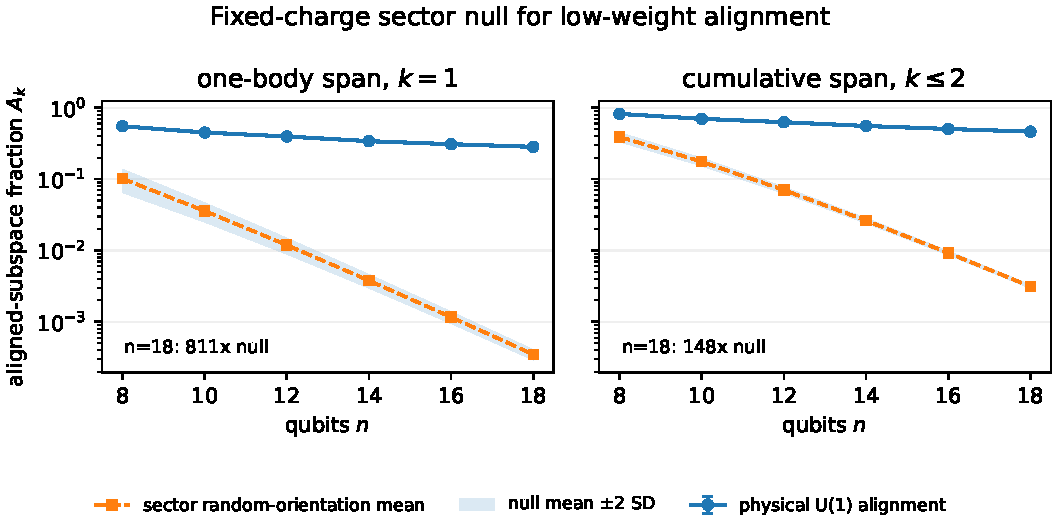
\includegraphics[width=.94\textwidth]{production/fig_u1_sector_null.pdf}
\caption{Sector-corrected random-orientation control for the half-filled $U(1)$ alignment statistic. The null draws the leading rank-$r_1$ subspace randomly inside the same fixed-charge centered score sector. Measured cross-fitted low-weight alignment remains far above this sector-corrected reference at the largest sizes, showing that the structured result is not produced by support or rank reduction alone.}
\label{fig:u1-aqt}
\end{figure*}

\section{The Separation Occurs at the Readout Stage}

The complete computational-basis record retains a similar order-one fraction of QFI in the generic and $U(1)$ circuits. Across the generic data, $F_{\mathrm{full}}/F_Q$ is approximately $0.49$, while the $U(1)$ values remain near $0.47$--$0.48$ \cite{AitHaddou2026MeasurementAccessible}. The large difference between these circuit classes emerges after projection onto the low-weight readout span. The structured $U(1)$ family does not simply preserve much more Fisher information under the computational-basis measurement; a larger fraction of its measured tangent information is oriented toward the retained low-weight functions.

\section{Discussion}

The experiments distinguish readout dimension from the geometry carried inside that dimension. Random orientation fixes the reference mean $r/N$, while the covariance spectrum sets the expected fluctuation scale around this value. A physical readout may nevertheless be preferentially aligned or misaligned with the dominant tangent eigenspaces. The generic and $U(1)$ circuits occupy different parts of this spectrum of behavior.

The equal-rank intervention provides the cleanest evidence. The circuit, measurement record, readout rank, evaluation tangents, and evaluation shot budget remain fixed. Replacing the physical Haar-$U(4)$ one-body span with a cross-fitted leading tangent subspace changes only which score directions are retained, yet the directional gradient-energy proxy increases by a factor of $9.584$ at $n=12$ and the finite-shot signal-to-noise ratio increases by $3.111$. The random rank-matched control stays near the physical baseline. These observations identify orientation, rather than rank alone, as the variable responsible for the difference.

The relation to adjacent work is correspondingly specific. Random-measurement results concern changes of the measurement basis and the recovery of quantum Fisher geometry after averaging \cite{LuSha2025}. Pauli-transfer analyses of quantum extreme learning machines concern the decodability of input-dependent Pauli features through reservoir dynamics and selected observables \cite{GrossRieser2026}. The present construction holds the measurement fixed and studies the covariance of trainable parameter tangents in the resulting classical score space. Standard Grassmann moments and the Ky Fan principle provide the null and upper benchmarks; the contribution lies in the covariance-resolved VQC formulation and the equal-rank operational controls.

The $U(1)$ case shows why a rank-only description is incomplete outside isotropy. After the null is restricted to the fixed-charge score sector, the leading tangent subspace remains strongly concentrated in low-weight diagonal sectors. The symmetry-breaking pilot is consistent with a role for exact conservation, but the present data do not identify a unique mechanism. This distinction is important because symmetry-restricted controllability, low-degree structure on a fixed-charge slice, readout compatibility with the conserved density, and slow operator dynamics make different predictions and require different interventions \cite{Monbroussou2025,Fontana2024,Ragone2024,Filmus2016,Khemani2018,Rakovszky2018}.

The analysis also has defined limits. It concerns local parameter tangents and a fixed computational-basis measurement. The principal readouts are diagonal and linear in the measurement record. Learning an aligned subspace requires calibration resources that are not included in the fixed evaluation-shot comparison. Finally, measurement-accessible tangent information is not equivalent to supervised task utility. A loss function may use only part of the accessible geometry, and optimization further depends on conditioning, noise, classical postprocessing, and the trajectory through parameter space. Those algorithmic questions are separate from the geometric claim tested here.

For quantum-technology design, the immediate implication is at the measurement/classical interface. Once a measurement record has been acquired, choosing a readout by dimension alone can discard directions that dominate the measurement-induced parameter geometry. Symmetry-adapted observables or calibrated readout subspaces can instead be assessed by their spectral orientation. Whether the gain justifies the calibration cost is an implementation-dependent resource question rather than a consequence of rank alone.

\section{Conclusion}

At fixed quantum measurement and fixed readout rank, the amount of accessible parameter-tangent information depends on which score directions the readout retains. Generic variational circuits can exhibit near-rank retention while their tangent covariance is strongly anisotropic, so agreement with a rank reference does not imply isotropy. In Haar-$U(4)$ circuits, a same-rank cross-fitted aligned subspace retains substantially more tangent mass than the physical one-body readout and produces larger finite-shot directional signal. A half-filled $U(1)$ circuit provides the complementary regime in which low-weight readouts are already strongly aligned with the leading tangent subspace after a sector-corrected comparison. Readout orientation is therefore a measurable design variable of the interface between quantum measurement and classical processing.

\bmsubsection*{Acknowledgments}
The author thanks Mohamed Bennai for helpful discussions.

\bmsubsection*{Artificial Intelligence Disclosure}
ChatGPT (OpenAI) was used during manuscript preparation to assist with language editing, structural revision, comparison against journal author guidelines, drafting of alternative prose, and preparation of an original schematic Table-of-Contents graphic. It was not used to generate, alter, or analyze the original research data or numerical results. The author checked the scientific claims, equations, citations, reported numerical values, and schematic content against the research record and takes full responsibility for the manuscript.

\bmsubsection*{Data Availability Statement}
The frozen numerical protocols, source code, aggregate tables, shard-level outputs, analysis scripts, and paper-facing result summaries supporting this study are available in the public project repository cited with the manuscript. A frozen AQT release is being prepared for archival in Zenodo; the final deposited DOI will be inserted before submission.

\bmsubsection*{Conflicts of Interest}
The author declares no conflict of interest.

\bmsubsection*{Funding}
The author received no specific funding for this work.

\bmsubsection*{Table of Contents Text}
This study shows that readouts of the same quantum measurement and the same dimension can expose very different parameter-tangent geometry. By comparing physical, random, and cross-fitted readouts at fixed rank, it isolates spectral orientation as the controlling variable and links that orientation to finite-shot directional signal, with a number-conserving circuit providing a structured high-alignment regime.

\clearpage
\begin{thebibliography}{99}

\bibitem{BraunsteinCaves1994}
S. L. Braunstein and C. M. Caves,
``Statistical Distance and the Geometry of Quantum States,''
Physical Review Letters \textbf{72}, 3439 (1994), doi:10.1103/PhysRevLett.72.3439.

\bibitem{Stokes2020}
J. Stokes, J. Izaac, N. Killoran, and G. Carleo,
``Quantum Natural Gradient,''
Quantum \textbf{4}, 269 (2020), doi:10.22331/q-2020-05-25-269.

\bibitem{Haug2021}
T. Haug, K. Bharti, and M. S. Kim,
``Capacity and Quantum Geometry of Parametrized Quantum Circuits,''
PRX Quantum \textbf{2}, 040309 (2021), doi:10.1103/PRXQuantum.2.040309.

\bibitem{HottaOzawa2004}
M. Hotta and M. Ozawa,
``Quantum Estimation by Local Observables,''
Physical Review A \textbf{70}, 022327 (2004), doi:10.1103/PhysRevA.70.022327.

\bibitem{LuLuoOh2012}
X.-M. Lu, S. Luo, and C. H. Oh,
``Hierarchy of Measurement-Induced Fisher Information for Composite States,''
Physical Review A \textbf{86}, 022342 (2012), doi:10.1103/PhysRevA.86.022342.

\bibitem{GrossRieser2026}
M. Gross and H.-M. Rieser,
``Theory and Interpretability of Quantum Extreme Learning Machines: A Pauli-Transfer Matrix Approach,''
arXiv:2602.18377 [quant-ph] (2026).

\bibitem{AitHaddou2026IsotropicRankLaws}
M. Ait Haddou,
``Readout-Rank Laws for Isotropic Quantum Tangents,''
arXiv:2608.07628 [quant-ph] (2026).

\bibitem{CollinsMatsumoto2017}
B. Collins and S. Matsumoto,
``Weingarten Calculus via Orthogonality Relations: New Applications,''
ALEA Latin American Journal of Probability and Mathematical Statistics \textbf{14}, 631 (2017), doi:10.30757/ALEA.v14-31.

\bibitem{Bendokat2024}
T. Bendokat, R. Zimmermann, and P.-A. Absil,
``A Grassmann Manifold Handbook: Basic Geometry and Computational Aspects,''
Advances in Computational Mathematics \textbf{50}, 6 (2024), doi:10.1007/s10444-023-10090-8.

\bibitem{KyFan1949}
K. Fan,
``On a Theorem of Weyl Concerning Eigenvalues of Linear Transformations I,''
Proceedings of the National Academy of Sciences of the United States of America \textbf{35}, 652 (1949), doi:10.1073/pnas.35.11.652.

\bibitem{Bergholm2018}
V. Bergholm, J. Izaac, M. Schuld, et al.,
``PennyLane: Automatic Differentiation of Hybrid Quantum-Classical Computations,''
arXiv:1811.04968 (2018).

\bibitem{AitHaddou2026MeasurementAccessible}
M. Ait Haddou,
``Spectral Geometry of Accessible Quantum Tangents: Reproducibility Repository,''
GitHub repository (2026),
\url{https://github.com/AHDMarwan/Spectral-Geometry-of-Accessible-Quantum-Tangents-Beyond-Isotropic-Readout-Rank-Laws}.

\bibitem{Efron1979}
B. Efron,
``Bootstrap Methods: Another Look at the Jackknife,''
The Annals of Statistics \textbf{7}, 1 (1979), doi:10.1214/aos/1176344552.

\bibitem{LuSha2025}
J. Lu and K. Sha,
``Quantum Fisher Information Matrix via Its Classical Counterpart from Random Measurements,''
arXiv:2509.08196 (2025).

\bibitem{Monbroussou2025}
L. Monbroussou, E. Z. Mamon, J. Landman, et al.,
``Trainability and Expressivity of Hamming-Weight Preserving Quantum Circuits for Machine Learning,''
Quantum \textbf{9}, 1745 (2025), doi:10.22331/q-2025-05-15-1745.

\bibitem{Fontana2024}
E. Fontana, D. Herman, S. Chakrabarti, et al.,
``Characterizing Barren Plateaus in Quantum Ans\"atze with the Adjoint Representation,''
Nature Communications \textbf{15}, 7171 (2024), doi:10.1038/s41467-024-49910-w.

\bibitem{Ragone2024}
M. Ragone, B. N. Bakalov, F. Sauvage, et al.,
``A Lie Algebraic Theory of Barren Plateaus for Deep Parameterized Quantum Circuits,''
Nature Communications \textbf{15}, 7172 (2024), doi:10.1038/s41467-024-49909-3.

\bibitem{Filmus2016}
Y. Filmus,
``An Orthogonal Basis for Functions over a Slice of the Boolean Hypercube,''
The Electronic Journal of Combinatorics \textbf{23}(1), P1.23 (2016), doi:10.37236/4567.

\bibitem{Khemani2018}
V. Khemani, A. Vishwanath, and D. A. Huse,
``Operator Spreading and the Emergence of Dissipative Hydrodynamics under Unitary Evolution with Conservation Laws,''
Physical Review X \textbf{8}, 031057 (2018), doi:10.1103/PhysRevX.8.031057.

\bibitem{Rakovszky2018}
T. Rakovszky, F. Pollmann, and C. W. von Keyserlingk,
``Diffusive Hydrodynamics of Out-of-Time-Ordered Correlators with Charge Conservation,''
Physical Review X \textbf{8}, 031058 (2018), doi:10.1103/PhysRevX.8.031058.

\end{thebibliography}

\clearpage
\setcounter{section}{0}
\setcounter{figure}{0}
\setcounter{table}{0}
\setcounter{equation}{0}
\renewcommand{\thesection}{S\arabic{section}}
\renewcommand{\thefigure}{S\arabic{figure}}
\renewcommand{\thetable}{S\arabic{table}}
\renewcommand{\theequation}{S\arabic{equation}}

\begin{center}
{\Large\bfseries Supporting Information}\\[6pt]
{\large Spectral Orientation of Measurement-Accessible Quantum Tangent Geometry in Variational Quantum Circuits}\\[8pt]
Marwan Ait Haddou\\
Independent Researcher\\
\texttt{aithaddou.marwan@outlook.com}
\end{center}

\section{Score-space construction and Fisher normalization}

Let $p_\theta(x)$ be the probability of outcome $x$ under the fixed computational-basis measurement and let $v$ be a parameter-space direction. The directional probability tangent is $\partial_v p_\theta(x)$. On the regular support, the Fisher-weighted tangent is
\begin{equation}
 s_v(x)=\frac{\partial_v p_\theta(x)}{\sqrt{p_\theta(x)}}.
\label{eq:si-score}
\end{equation}
The probability-normalization constraint removes the constant mode, leaving an $N$-dimensional centered real score space. Each regular tangent direction is normalized as
\begin{equation}
 u_v=\frac{s_v}{\|s_v\|_2},\qquad \|u_v\|_2=1,
\label{eq:si-normalized-score}
\end{equation}
and the tangent covariance is
\begin{equation}
 C=\mathbb E_v[u_vu_v^{\mathsf T}],\qquad \Tr C=1.
\label{eq:si-C}
\end{equation}
Before the normalization in Eq.~\eqref{eq:si-normalized-score}, $\|s_v\|_2^2$ is the classical Fisher information carried by the fixed measurement along $v$ \cite{BraunsteinCaves1994,LuLuoOh2012}. The normalized covariance therefore records the distribution of measurement-visible tangent directions after factoring out their overall Fisher scale.

For an orthogonal readout projector $P$,
\begin{align}
\mathbb E_v\|Pu_v\|_2^2
&=\mathbb E_v\,u_v^{\mathsf T}Pu_v \\
&=\Tr\!\left(P\,\mathbb E_v[u_vu_v^{\mathsf T}]\right)
=\Tr(PC),
\label{eq:si-R}
\end{align}
which is the retained tangent mass used in the main article.

\section{Grassmann random-orientation moments}

Let $P$ be Haar-uniform on the real Grassmann manifold $\mathrm{Gr}(r,N)$. Orthogonal invariance gives
\begin{equation}
\mathbb E P=\frac rN I,
\end{equation}
so that for any trace-one covariance $C$,
\begin{equation}
\mathbb E\Tr(PC)=\frac rN.
\end{equation}
The second moment of a random orthogonal projector has the invariant form
\begin{equation}
\mathbb E[P_{ij}P_{kl}]
=a\,\delta_{ij}\delta_{kl}
+b\,(\delta_{ik}\delta_{jl}+\delta_{il}\delta_{jk}),
\label{eq:si-projector-second}
\end{equation}
with coefficients determined by $P^2=P$ and $\Tr P=r$ \cite{CollinsMatsumoto2017}. Contracting Eq.~\eqref{eq:si-projector-second} with $C_{ji}C_{lk}$ gives
\begin{equation}
\operatorname{Var}[\Tr(PC)]
=\frac{2r(N-r)}{N^2(N-1)(N+2)}
\left[N\Tr(C^2)-1\right].
\label{eq:si-var-R}
\end{equation}
For $\rho=N\Tr(PC)/r$,
\begin{equation}
\operatorname{Var}(\rho)
=\frac{2(N-r)[N\Tr(C^2)-1]}
{r(N-1)(N+2)}.
\label{eq:si-var-rho}
\end{equation}
Using $N-r\le N-1$ and $N\Tr(C^2)-1\le (N+2)\Tr(C^2)$ gives
\begin{equation}
\operatorname{Var}(\rho)\le \frac{2}{r d_{\rm eff}},
\qquad d_{\rm eff}=\frac1{\Tr(C^2)}.
\label{eq:si-deff-bound}
\end{equation}
Thus concentration near the rank reference depends on $r d_{\rm eff}$ and does not require $d_{\rm eff}/N$ to approach one.

\begin{figure*}[t]
\centering
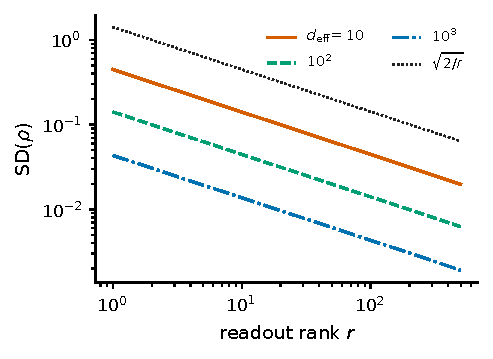
\includegraphics[width=.76\textwidth]{figS2_exact_null_width.pdf}
\caption{Exact random-orientation fluctuation scale for representative effective dimensions. The standard deviation of $\rho$ narrows with increasing readout rank and effective spectral dimension while remaining compatible with a strongly anisotropic covariance when $r d_{\rm eff}$ is large.}
\label{fig:si-null-width}
\end{figure*}

\section{Fixed-weight diagonal readout spaces}

For full computational-basis support, the centered outcome space has dimension $N=2^n-1$. Distinct nonidentity diagonal Pauli strings are orthogonal in the uniform Walsh basis, so the cumulative weight-through-$k$ span has dimension
\begin{equation}
 r_{\le k}=\sum_{j=1}^k\binom nj.
\label{eq:si-rank-full}
\end{equation}
For fixed $k$ and large $n$, $r_{\le k}=n^k/k!\,[1+O(n^{-1})]$.

In the half-filled fixed-charge sector, the outcome support contains $\binom{n}{n/2}$ basis strings and the centered score dimension is
\begin{equation}
 N_{\rm hf}=\binom{n}{n/2}-1.
\end{equation}
The identity $\sum_i Z_i=0$ on the half-filled support removes one one-body degree of freedom, giving
\begin{equation}
 r_1=n-1.
\end{equation}
For the cumulative one- and two-body diagonal span, the centered dimension used in the numerical protocol is
\begin{equation}
 r_{\le2}=\binom n2-1.
\end{equation}
These rank identities provide geometric bookkeeping and do not determine the physical orientation of the tangent covariance. Fixed-charge harmonic analysis provides broader mathematical context for low-degree functions on a slice \cite{Filmus2016}.

\begin{figure*}[t]
\centering
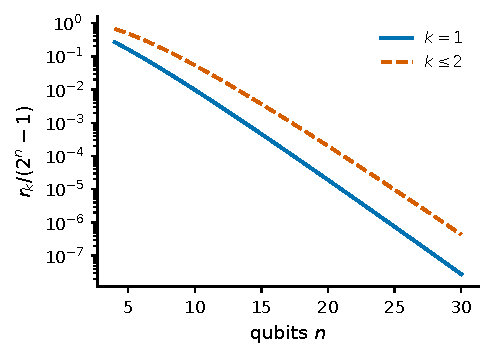
\includegraphics[width=.76\textwidth]{figS4_rank_fraction.pdf}
\caption{Rank fractions for low-weight diagonal readouts under full computational-basis support. Polynomially growing low-weight spaces occupy an exponentially shrinking fraction of the centered record.}
\label{fig:si-rank-fractions}
\end{figure*}

\section{Cross-fitting, Ky Fan benchmark, and statistical unit}

For a covariance estimate $\widehat C_{\rm fit}$ obtained from one tangent ensemble, let $Q_r$ contain its leading $r$ eigenvectors and define
\begin{equation}
P_{\rm xfit}=Q_rQ_r^{\mathsf T}.
\end{equation}
Retention is evaluated on an independent tangent ensemble,
\begin{equation}
 R_{\rm xfit}=\frac1{m_{\rm eval}}\sum_{a=1}^{m_{\rm eval}}
\|P_{\rm xfit}u_a^{\rm(eval)}\|_2^2.
\label{eq:si-crossfit}
\end{equation}
This prevents the same tangent samples from both selecting and evaluating the subspace. The frozen operational profile uses 128 alignment tangents and 128 independent evaluation tangents per circuit. The generic Haar-$U(4)$ cells use 16 circuit instances per size and the $U(1)$ cells use 20, with a 10,000-shot finite-shot evaluation model and 8 held-out finite-difference directions. The alignment sample is a separate calibration resource and is not counted as free measurement cost in the fixed-evaluation-budget comparison.

The same-sample Ky Fan quantity
\begin{equation}
R_{\rm KF}=\sum_{j=1}^r\lambda_j(\widehat C)
\end{equation}
is an optimistic spectral upper benchmark rather than the operational estimator \cite{KyFan1949}. The independent resampling unit throughout the statistical analysis is the circuit instance. Confidence intervals resample circuit instances and recompute the relevant aggregate. Frozen profiles, deterministic seeds, shard-level outputs, and paper-facing summaries are archived in the reproducibility repository \cite{AitHaddou2026MeasurementAccessible}.

\section{Finite-shot directional-signal diagnostics}

Let $F_{\rm full}(v)$ denote the classical Fisher scale of direction $v$ before unit normalization. For rank-$r$ projector $P$, define
\begin{equation}
E_{\rm raw}(P)=\mathbb E_v\!\left[F_{\rm full}(v)\,\|Pu_v\|_2^2\right].
\label{eq:si-raw-energy}
\end{equation}
If a scalar readout direction is sampled isotropically inside the retained $r$-dimensional subspace, the mean squared directional signal is
\begin{equation}
\mathbb E[g_{\rm dir}^2]=\frac{E_{\rm raw}(P)}{r}.
\label{eq:si-dir-signal}
\end{equation}
The finite-shot calculation combines this signal with the multinomial covariance of the fixed measurement record. Physical, random-rank, and aligned comparisons keep the circuit, quantum measurement, readout rank, and shot count fixed. These are controlled directional diagnostics, not gradient-variance claims for an arbitrary supervised loss.

\begin{figure*}[t]
\centering
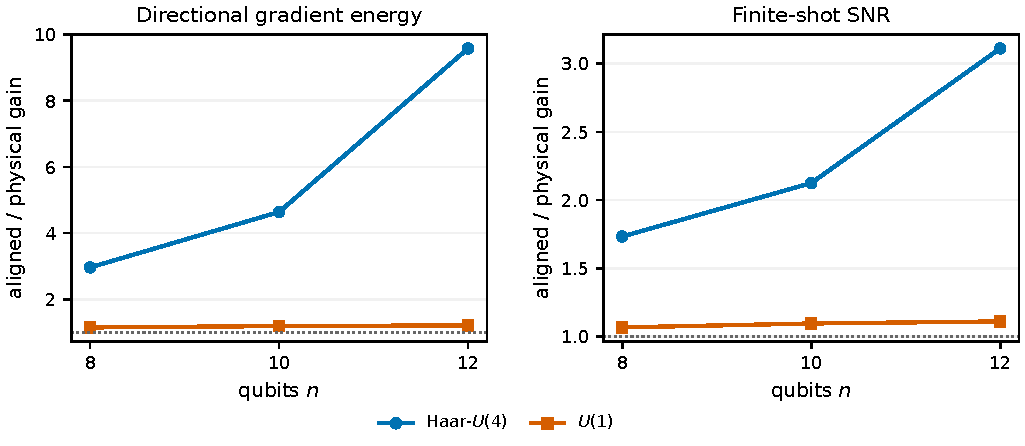
\includegraphics[width=.90\textwidth]{appendix_operational_gains.pdf}
\caption{Additional fixed-rank operational diagnostics. Retention, directional gradient-energy, and finite-shot SNR gains are shown for the physical versus cross-fitted aligned comparison. Generic Haar-$U(4)$ circuits leave substantial room for orientation improvement, whereas the structured $U(1)$ readout is already comparatively aligned.}
\label{fig:si-operational}
\end{figure*}

\section{Additional covariance, orientation, and readout-noise diagnostics}

\begin{figure*}[t]
\centering
\begin{minipage}{.32\textwidth}\centering
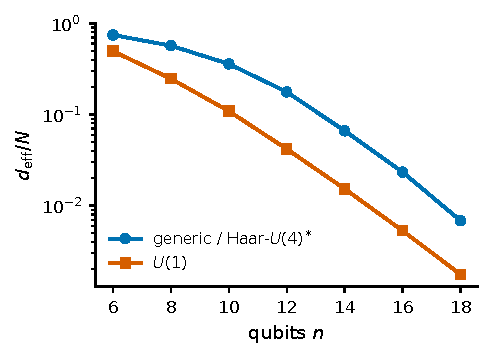
\includegraphics[width=\linewidth]{figS1_deff_fraction.pdf}
\end{minipage}\hfill
\begin{minipage}{.32\textwidth}\centering
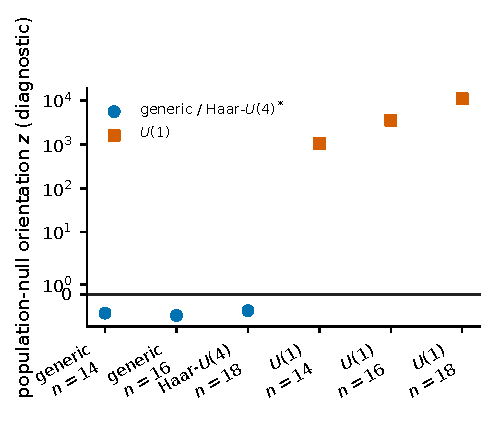
\includegraphics[width=\linewidth]{figS3_orientation_z.pdf}
\end{minipage}\hfill
\begin{minipage}{.32\textwidth}\centering
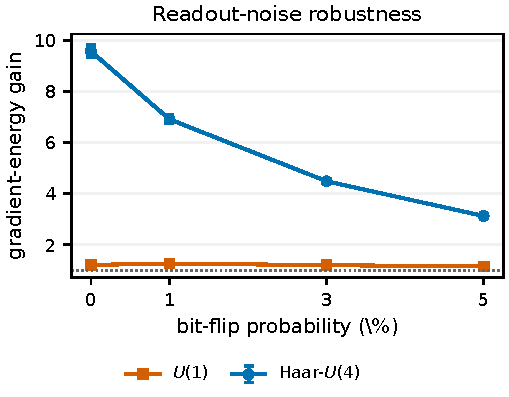
\includegraphics[width=\linewidth]{appendix_noise_robustness.pdf}
\end{minipage}
\caption{Supporting diagnostics. Left: effective spectral fraction $d_{\rm eff}/N$. Center: population-null orientation diagnostic for representative generic/Haar and $U(1)$ points. Right: aligned-to-physical directional gradient-energy gain under readout bit-flip noise. In the noise comparison the aligned subspace is re-estimated after noise is applied; the panel therefore does not establish robustness of one fixed optimized observable.}
\label{fig:si-supporting}
\end{figure*}

\section{Finite-size diagnostics for the half-filled $U(1)$ family}

Across $n=8,10,12,14,16,18$, the cross-fitted one-body overlaps are $0.552$, $0.450$, $0.396$, $0.341$, $0.309$, and $0.284$, respectively. At $n=18$,
\begin{equation}
A_1(18)=0.283586\;[0.277044,0.290865],
\end{equation}
and the cumulative weight-through-two overlap is
\begin{equation}
A_{\le2}(18)=0.463538\;[0.457425,0.469591].
\end{equation}
Each size uses 20 independent circuit instances. Two-parameter log-space model comparison over the tested window favors a power form over an exponential form. The fitted exponents are $0.8223\,[0.7694,0.8735]$ for $A_1$ and $0.7041\,[0.6798,0.7281]$ for $A_{\le2}$, with $\Delta\mathrm{AICc}=14.39$ and $12.82$, respectively, in favor of the power model. These results describe finite-size model discrimination only and are not asymptotic bounds or hydrodynamic exponents \cite{AitHaddou2026MeasurementAccessible}.

\begin{figure*}[t]
\centering
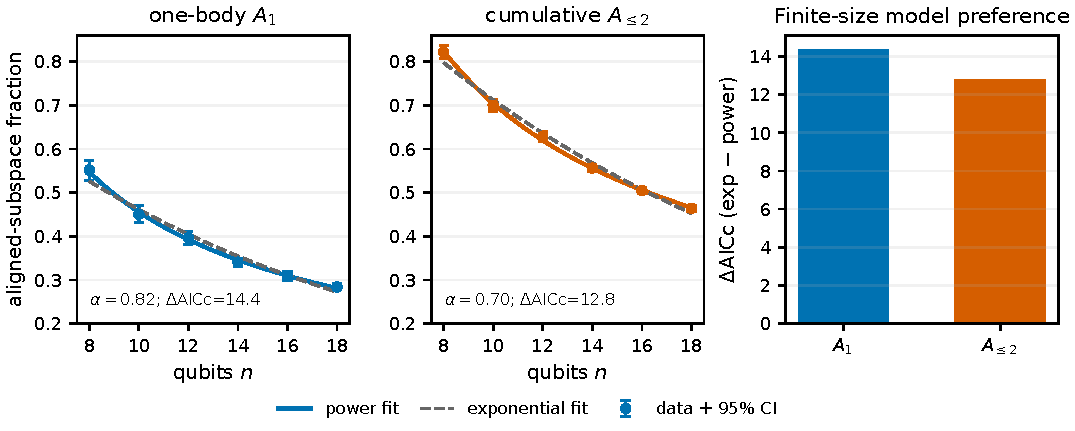
\includegraphics[width=.96\textwidth]{appendix_u1_fit_diagnostics.pdf}
\caption{Finite-size diagnostics for the half-filled $U(1)$ family. The plots compare the measured overlaps with power and exponential fits over $n=8$--$18$ and summarize $\Delta\mathrm{AICc}=\mathrm{AICc}_{\rm exp}-\mathrm{AICc}_{\rm power}$. Positive values favor the power model only within the tested window.}
\label{fig:si-u1-fits}
\end{figure*}

\section{Symmetry-breaking sensitivity control}

A separate $n=8$ pilot holds the trainable parameter count fixed while adding a nontrainable perturbation. The unperturbed one-body alignment is
\begin{equation}
A_1=0.517\;[0.486,0.549].
\end{equation}
A symmetry-preserving $R_Z$ perturbation of strength $\epsilon=0.3$ gives
\begin{equation}
A_1=0.481\;[0.454,0.518],
\end{equation}
whereas a symmetry-breaking $R_X$ perturbation at the same strength gives
\begin{equation}
A_1=0.0295\;[0.0248,0.0338].
\end{equation}
The physical one-body retention simultaneously falls from $0.430$ to $0.0325$ in the breaking control \cite{AitHaddou2026MeasurementAccessible}. This pilot establishes sensitivity to charge breaking in the tested setting; it does not identify which microscopic mechanism produces the unperturbed alignment.

\begin{figure*}[t]
\centering
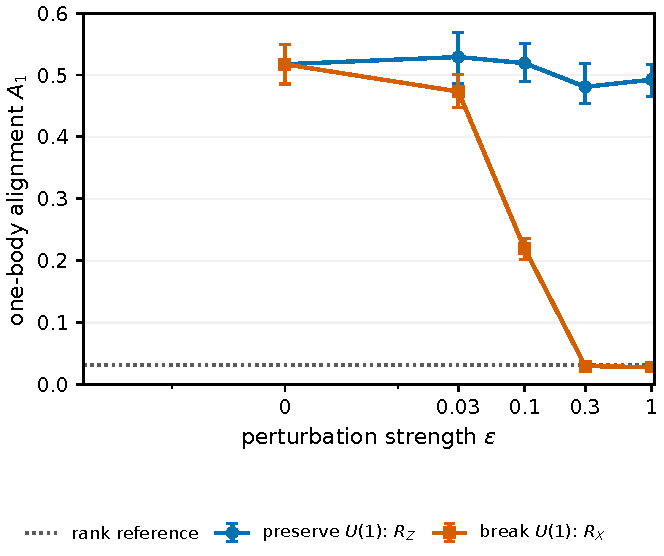
\includegraphics[width=.78\textwidth]{production/fig_symmetry_breaking_control.pdf}
\caption{Symmetry-breaking pilot at $n=8$. Symmetry-preserving $R_Z$ perturbations leave the one-body tangent-subspace overlap comparatively stable, whereas nontrainable $R_X$ perturbations that break charge conservation suppress it toward the full-score-space rank scale. Error bars are 95\% circuit-bootstrap intervals over 10 circuit instances.}
\label{fig:si-symmetry-breaking}
\end{figure*}

\section{Circuit conventions and reproducibility}

The numerical campaign uses RY--RZ--CZ, SU2--CNOT, SU2--CZ ring, SU2--CZ random-matching, Haar-$U(4)$ brickwork, and half-filled $U(1)$ RZ--XY circuit families. The PennyLane drawings below are schematics; parameter values are suppressed and representative layers are shown for legibility. Simulations use the exact gate constructors, depth conventions, deterministic seeds, and frozen experiment profiles archived in the repository \cite{Bergholm2018,AitHaddou2026MeasurementAccessible}.

\begin{figure*}[t]
\centering
\begin{minipage}{.32\textwidth}\centering
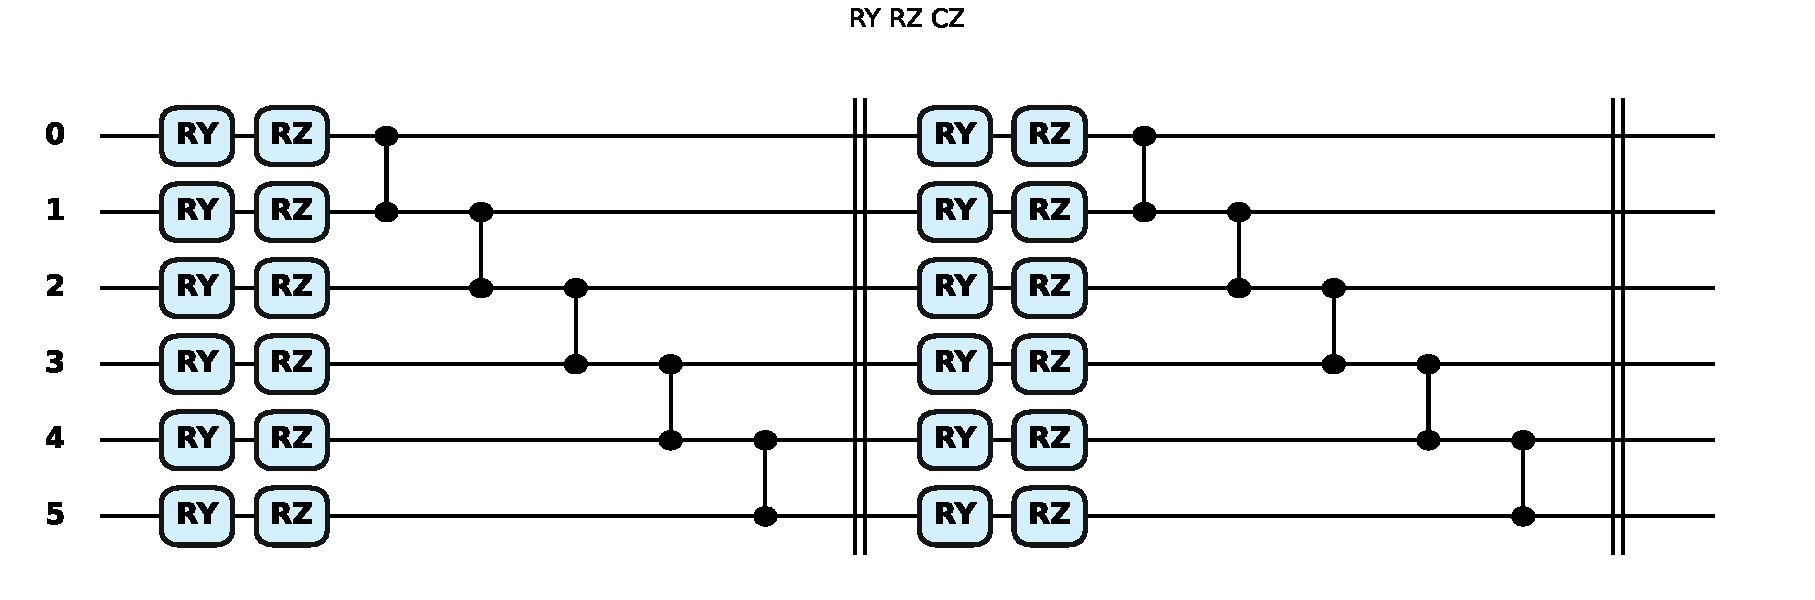
\includegraphics[width=\linewidth]{generated_circuits/circuit_ry_rz_cz.pdf}\\[-1mm]{\scriptsize RY--RZ--CZ}
\end{minipage}\hfill
\begin{minipage}{.32\textwidth}\centering
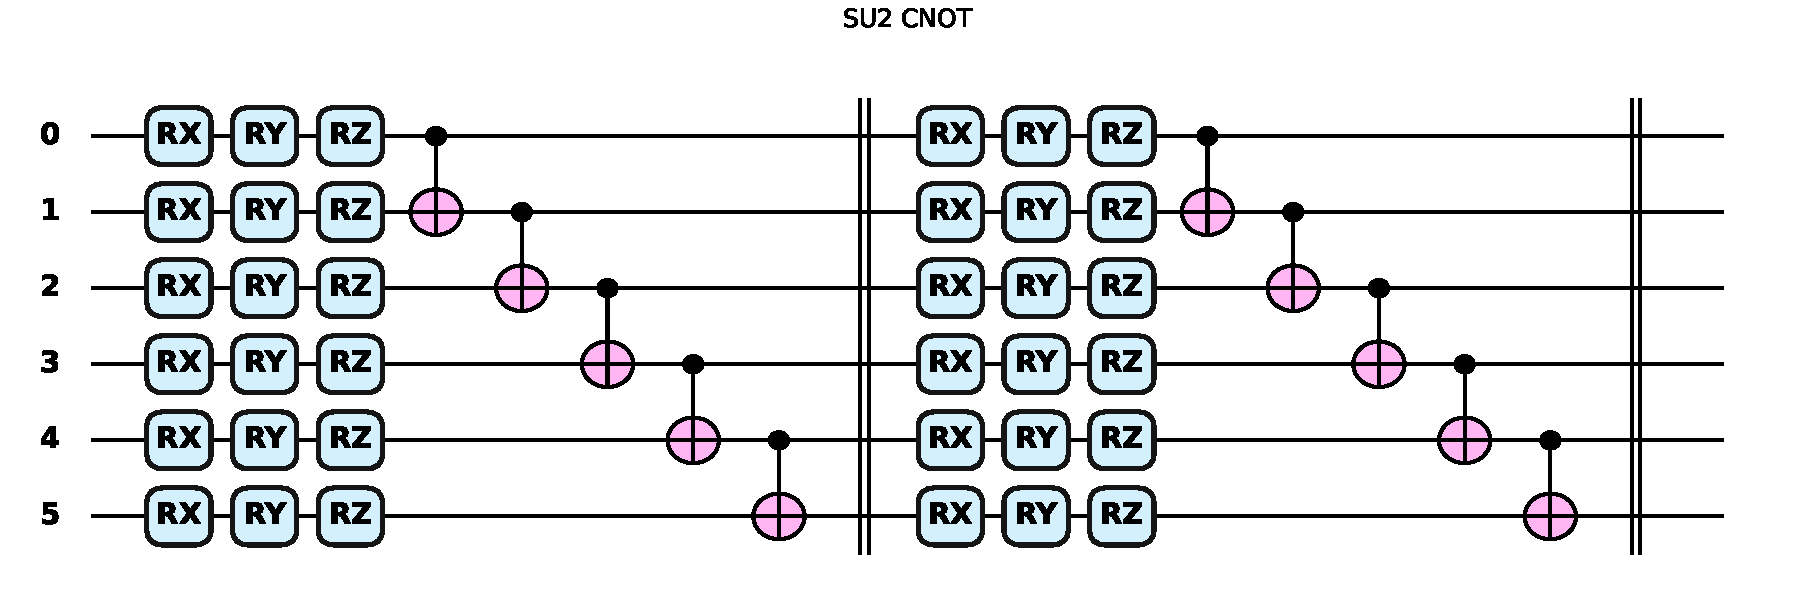
\includegraphics[width=\linewidth]{generated_circuits/circuit_su2_cnot.pdf}\\[-1mm]{\scriptsize SU2--CNOT}
\end{minipage}\hfill
\begin{minipage}{.32\textwidth}\centering
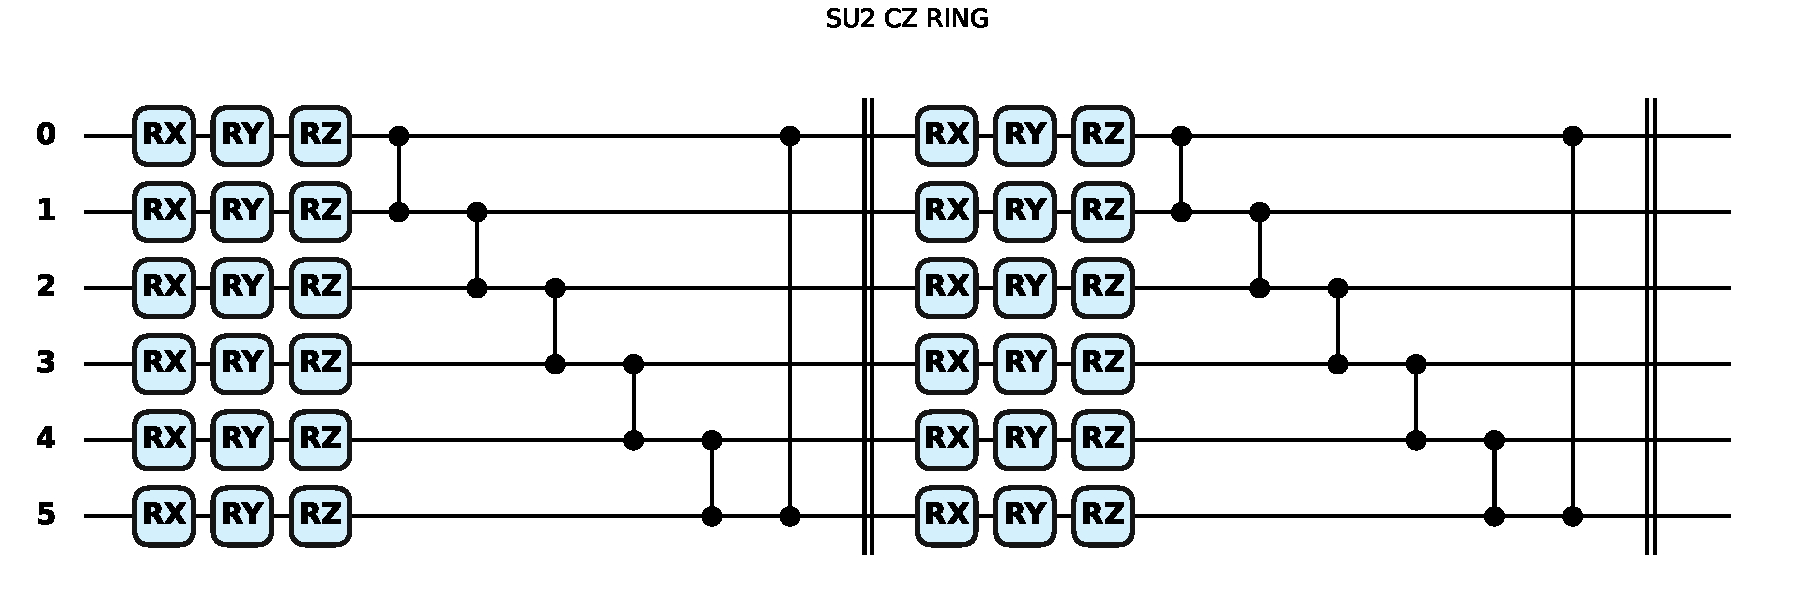
\includegraphics[width=\linewidth]{generated_circuits/circuit_su2_cz_ring.pdf}\\[-1mm]{\scriptsize SU2--CZ ring}
\end{minipage}
\vspace{2mm}
\begin{minipage}{.32\textwidth}\centering
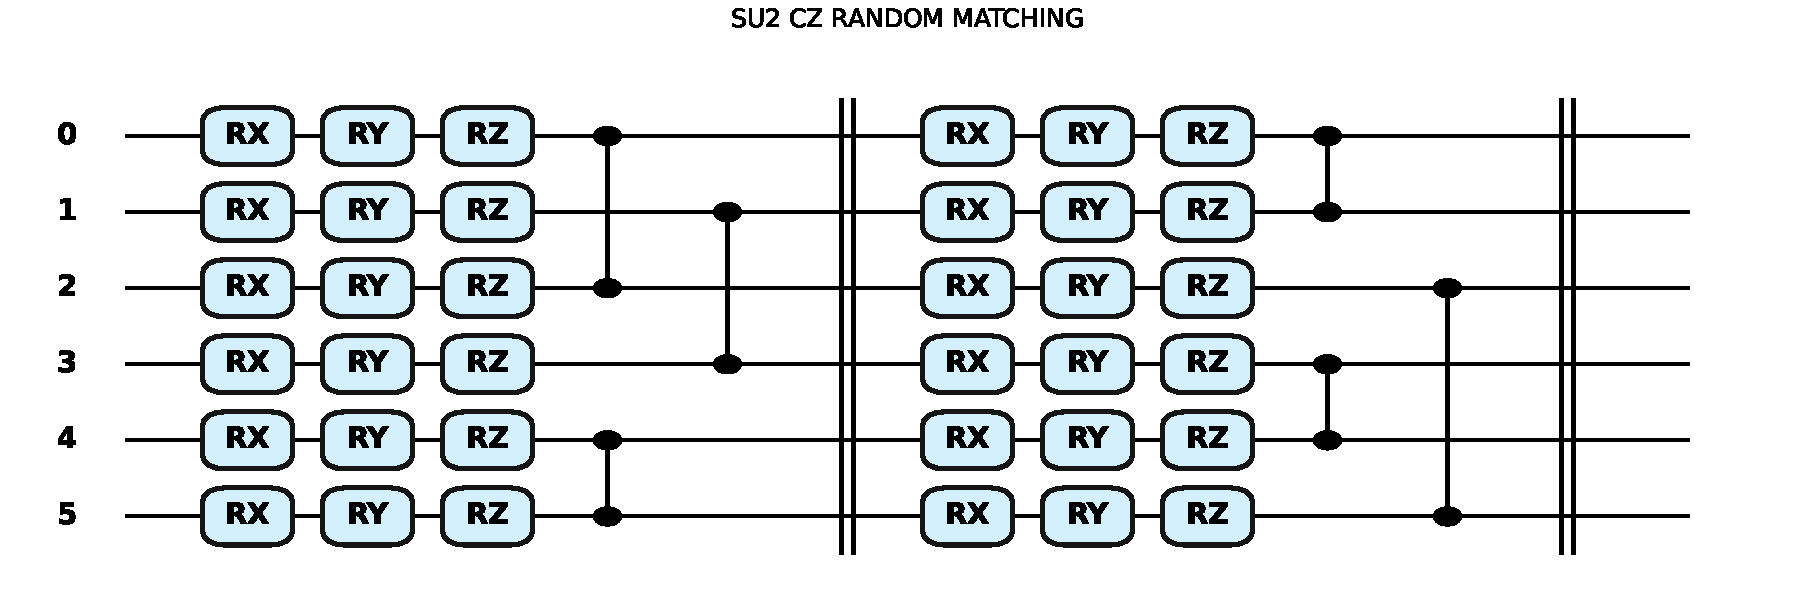
\includegraphics[width=\linewidth]{generated_circuits/circuit_su2_cz_random_matching.pdf}\\[-1mm]{\scriptsize SU2--CZ random matching}
\end{minipage}\hfill
\begin{minipage}{.32\textwidth}\centering
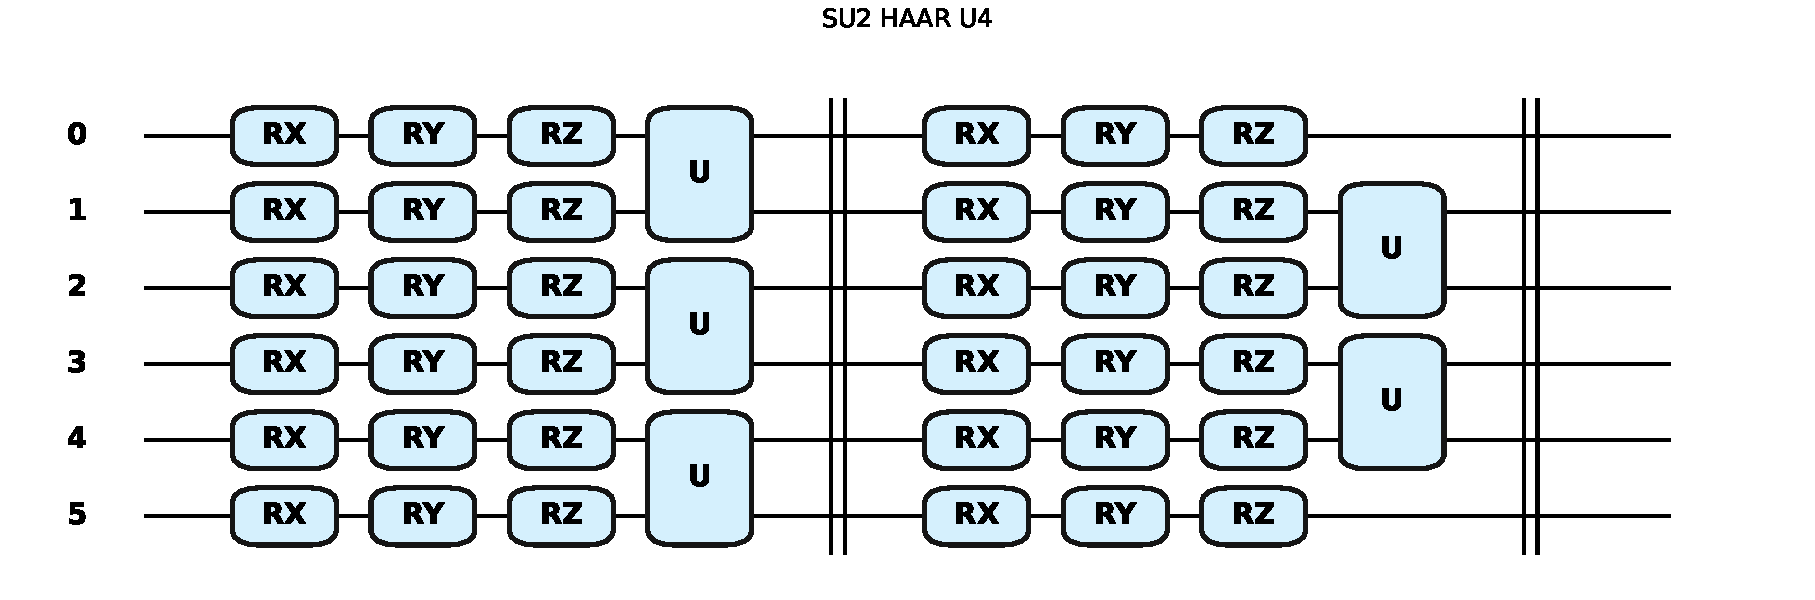
\includegraphics[width=\linewidth]{generated_circuits/circuit_su2_haar_u4.pdf}\\[-1mm]{\scriptsize Haar-$U(4)$ brickwork}
\end{minipage}\hfill
\begin{minipage}{.32\textwidth}\centering
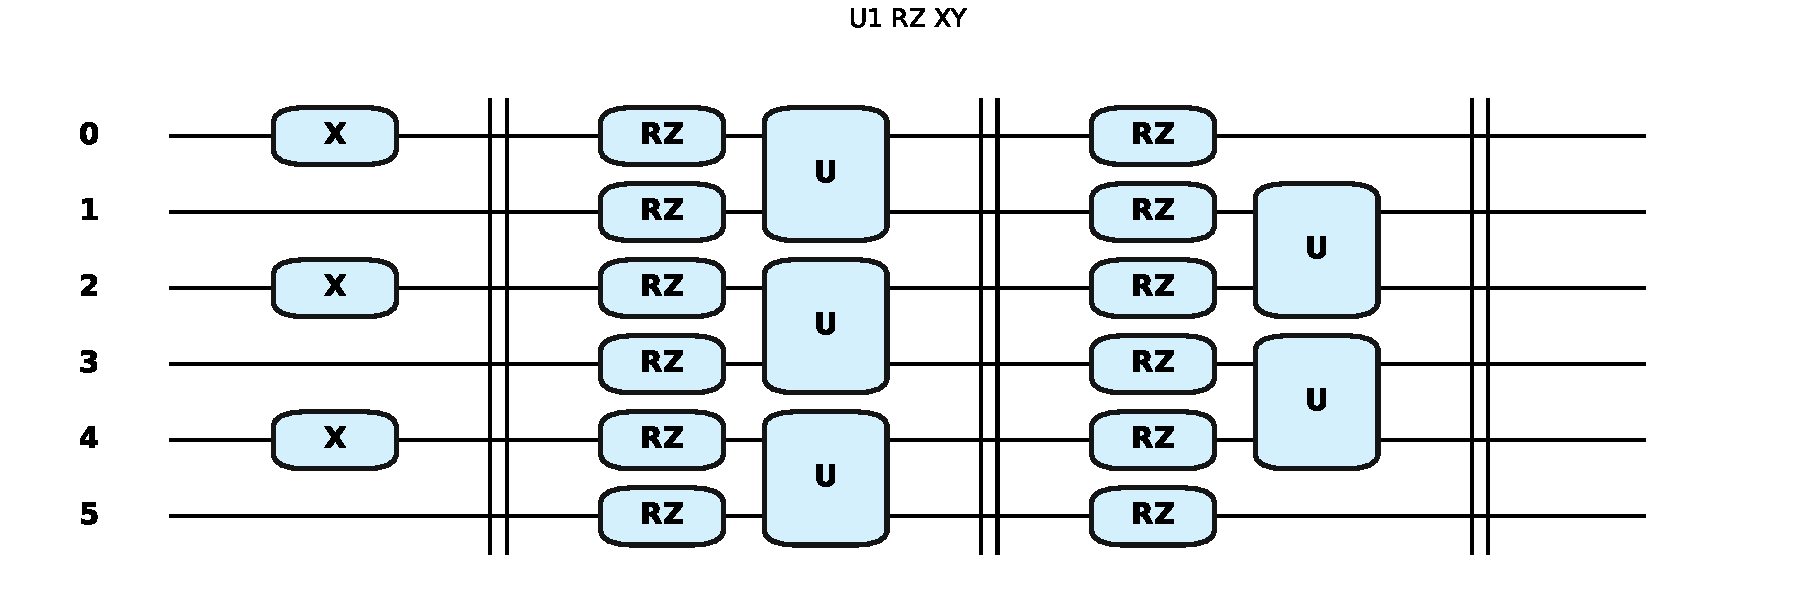
\includegraphics[width=\linewidth]{generated_circuits/circuit_u1_rz_xy.pdf}\\[-1mm]{\scriptsize half-filled $U(1)$ RZ--XY}
\end{minipage}
\caption{Circuit schematics corresponding to the families used in the numerical campaign.}
\label{fig:si-circuits}
\end{figure*}

\section{Data and code provenance}

The reproducibility repository contains frozen experiment profiles, source code, deterministic seeds, aggregate tables, shard-level outputs, analysis scripts, and the paper-facing summaries used for the numerical values in the main article and this Supporting Information \cite{AitHaddou2026MeasurementAccessible}. The AQT release candidate additionally includes \texttt{.zenodo.json} and \texttt{CITATION.cff} metadata for archival of the frozen repository release.

\end{document}
